\subsubsection*{Problem definition}

This test example is taken from the PHREEQC User's Guide (Parkhurst and Appelo, 1999), a manual for a computer program that is applicable for chemical reactions and transport processes. The simulation is made in order to reproduce the transport of solutes by saturated flow with the influence of cation exchange. The aim of the example is to check out the correctness of the coupling between GeoSys/RockFlow and PHREEQC by comparing the results of the simulations of both programs. With the calculation model the chemical composition of the effluent from a column containing a cation exchanger and a sodium-potassium-nitrate-solution is simulated. This column is flushed with 3 pore volumes of calcium chloride solution.

\textsl{Assumptions}

\begin{tabbing}
Components: \= calcium, potassium and sodium react to equilibrium with cation \\ \>exchanger at all times \\
Aquifer: \> homogeneous, saturated, stationary flow \\
\end{tabbing}

\subsubsection*{Model set-up of the 1~D numerical model}

The 8.2~cm long column contains a sodium-potassium-nitrate solution that is in equilibrium with a cation exchanger. For the one-dimensional calculation the calculation area is simplified as a line of a length of 8.2~cm. The calculation model includes 82 elements and 83 nodes. As initial condition the water head in the whole domain is given with 2~m. The initial state of the solution is given in table \ref{tab56}.

\begin{table}[htbp]
\centering
\begin{tabular}{|l|l|l|}
\hline
parameter & value & unit \\
\hline
Ca & 0 & -- \\
\hline
Cl & 0 & -- \\
\hline
K & 2.0$\cdot 10^{-4}$ & mol/kgw \\
\hline
Na & 1.0$\cdot 10^{-3}$ & mol/kgw \\
\hline
N(5) & 1.2$\cdot 10^{-3}$ & mol/kgw \\
\hline
pH & 7 & -- \\
\hline
pe & 12.5 & -- \\
\hline
Na-X & 5.493$\cdot 10^{-4}$ & mol/kgw \\
\hline
K-X & 5.507$\cdot 10^{-4}$ & mol/kgw \\
\hline
Ca-X$_2$ & 0 & -- \\
\hline
\end{tabular}
\caption{Used parameters}
\label{tab56}
\end{table}

{\small
with
\begin{tabbing}
\=xxxxxxx \=xxxxxxxxxxxxxxxxxx \kill
\> pe \> - redox potential \\
\> X \> - ion exchanger \\
\> kgw \> - kilogram of water. \\
\end{tabbing}
}

At the right border of the model the constant head is given with 2~m. At the left border a constant flux of 1.388$\cdot 10^{-6}$~m$^3$/s is defined as source term. The concentrations of this infiltrating CaCl$_2$-solution as well as the pH and pe are given in table \ref{tab57}.

\begin{table}[htbp]
\centering
\begin{tabular}{|l|l|l|}
\hline
parameter & value & unit \\
\hline
Ca & 6.0$\cdot 10^{-4}$ & mol/kgw \\
\hline
Cl & 1.2$\cdot 10^{-3}$ & mol/kgw \\
\hline
pH & 7 & -- \\
\hline
pe & 12.5 & -- \\
\hline
\end{tabular}
\caption{State of the infiltration solution}
\label{tab57}
\end{table}

The soil material is specified by the parameters in table \ref{tab58}. The dispersion of the transported solutes in this soil is set equal to 2$\cdot 10^{-3}$~m. The calculation is divided in 480 time steps with a constant time step length of 180 seconds. That means, the flow and transport processes in the aquifer within 1 day are simulated.

\begin{table}[htbp]
\centering
\begin{tabular}{|l|l|l|}
\hline
density $\rho$  & 2000 & kg/m$^{-3}$  \\
\hline
porosity $\Phi$ & 0.5 & -- \\
\hline
permeability $K$ & 1.157$\cdot 10^{-5}$ & m$^2$ \\
\hline
\end{tabular}
\caption{Soil parameters}
\label{tab58}
\end{table}

\subsubsection*{Evaluation method}
As this test example has the aim to validate the coupling of GeoSys/RockFlow and PHREEQC, merely the comparison between the simulation results of both programs has to be accomplished.


\begin{figure}[htbp]
\centering
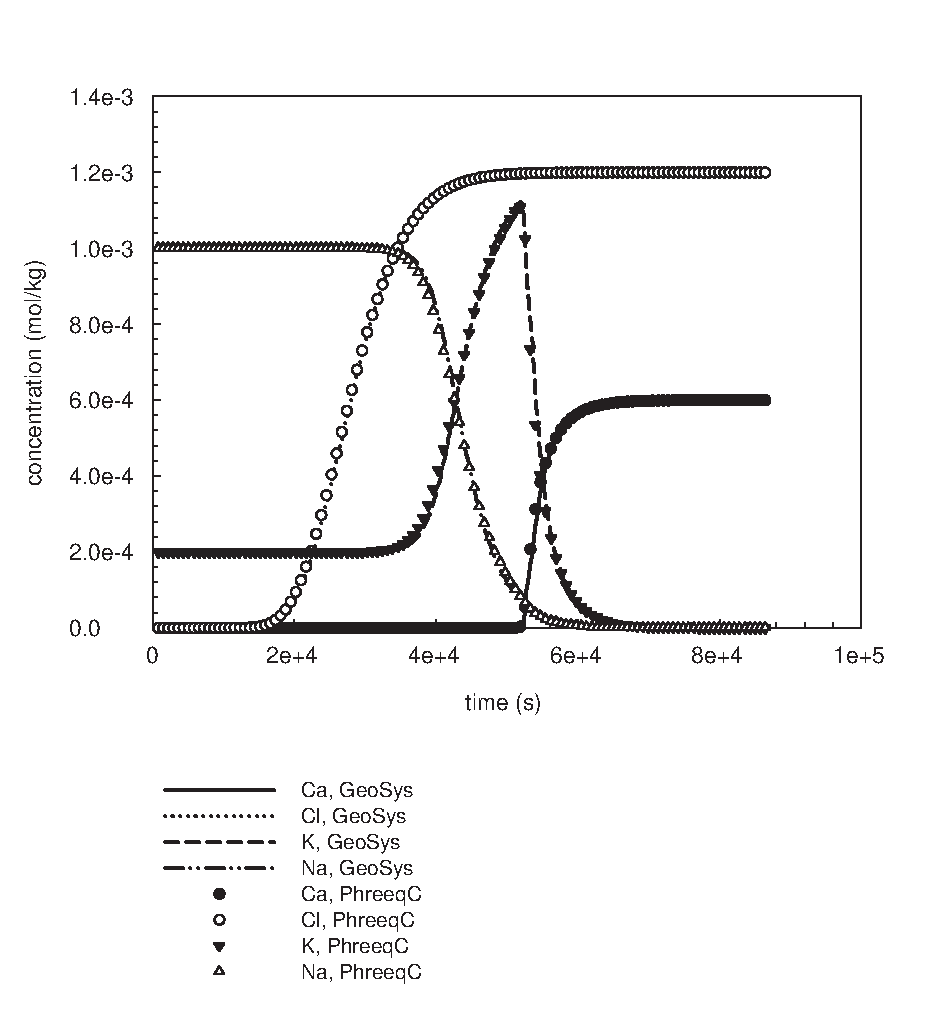
\includegraphics[width=0.8\textwidth]{C/figures/fig513.EPS}
\caption{Effluent concentrations  with time of the GeoSys/RockFlow and PHREEQC simulations}
\label{fig513}
\end{figure}

\subsubsection*{Results}

The numerical results are shown in figure \ref{fig513}. The time-dependent concentrations are the values of the compared GeoSys/RockFlow and PHREEQC models at the end node and end cell, respectively. Within the calculation time of one day the pore volume of the column model is exchanged three times. As chloride is a conservative tracer it arrives already after the exchange of about one pore volume in the effluent. As long as the exchanger contains sodium this component is eluted. Sodium is initially present in the column and exchanges with the incoming calcium. Potassium is released after sodium. When all of the potassium has been released, the concentration of calcium increases to a steady-state value. As depicted in figure \ref{fig513}, between the GeoSys/RockFlow and the PHREEQC simulation results there are no differences.

\begin{tabular}{|l|l|l|}
\hline
Benchmark & Problem type	& Path in benchmark deposit \\
\hline	
pqc1	& HC	& benchmarks $\backslash$HC$\backslash$ion\_exchange \\
\hline	
\end{tabular}
